\documentclass[answers]{exam}

\usepackage{amsmath}
\usepackage{amssymb}
\usepackage{geometry}
\usepackage{venndiagram}
\usepackage{graphics}
\usepackage{graphicx}
\usepackage{siunitx}

% Header and footer.
\pagestyle{headandfoot}
\runningheadrule
\runningfootrule
\runningheader{EE/CE 468/468 Mobile Robotics}{Homework 1}{Fall 2023}
\runningfooter{}{Page \thepage\ of \numpages}{}
\firstpageheader{}{}{}

\boxedpoints
\printanswers

\newcommand{\uvec}[1]{\boldsymbol{\hat{\textbf{#1}}}}
\newcommand\union\cup
\newcommand\inter\cap
\newcommand\ul\underline
\newcommand\ol\overline

\title{Homework 1\\ EE/CE 468/468 Mobile Robotics\\ Habib University -- Fall 2023}
\author{Ali Asghar Yousuf\\ Muhammad Azeem Haider}  % replace with your ID, e.g. oy02945
\date{\today}

\begin{document}
\maketitle

\begin{questions}
    \question Problem 1
    \begin{parts}
        \part Part a
        \begin{solution}

            \centering
            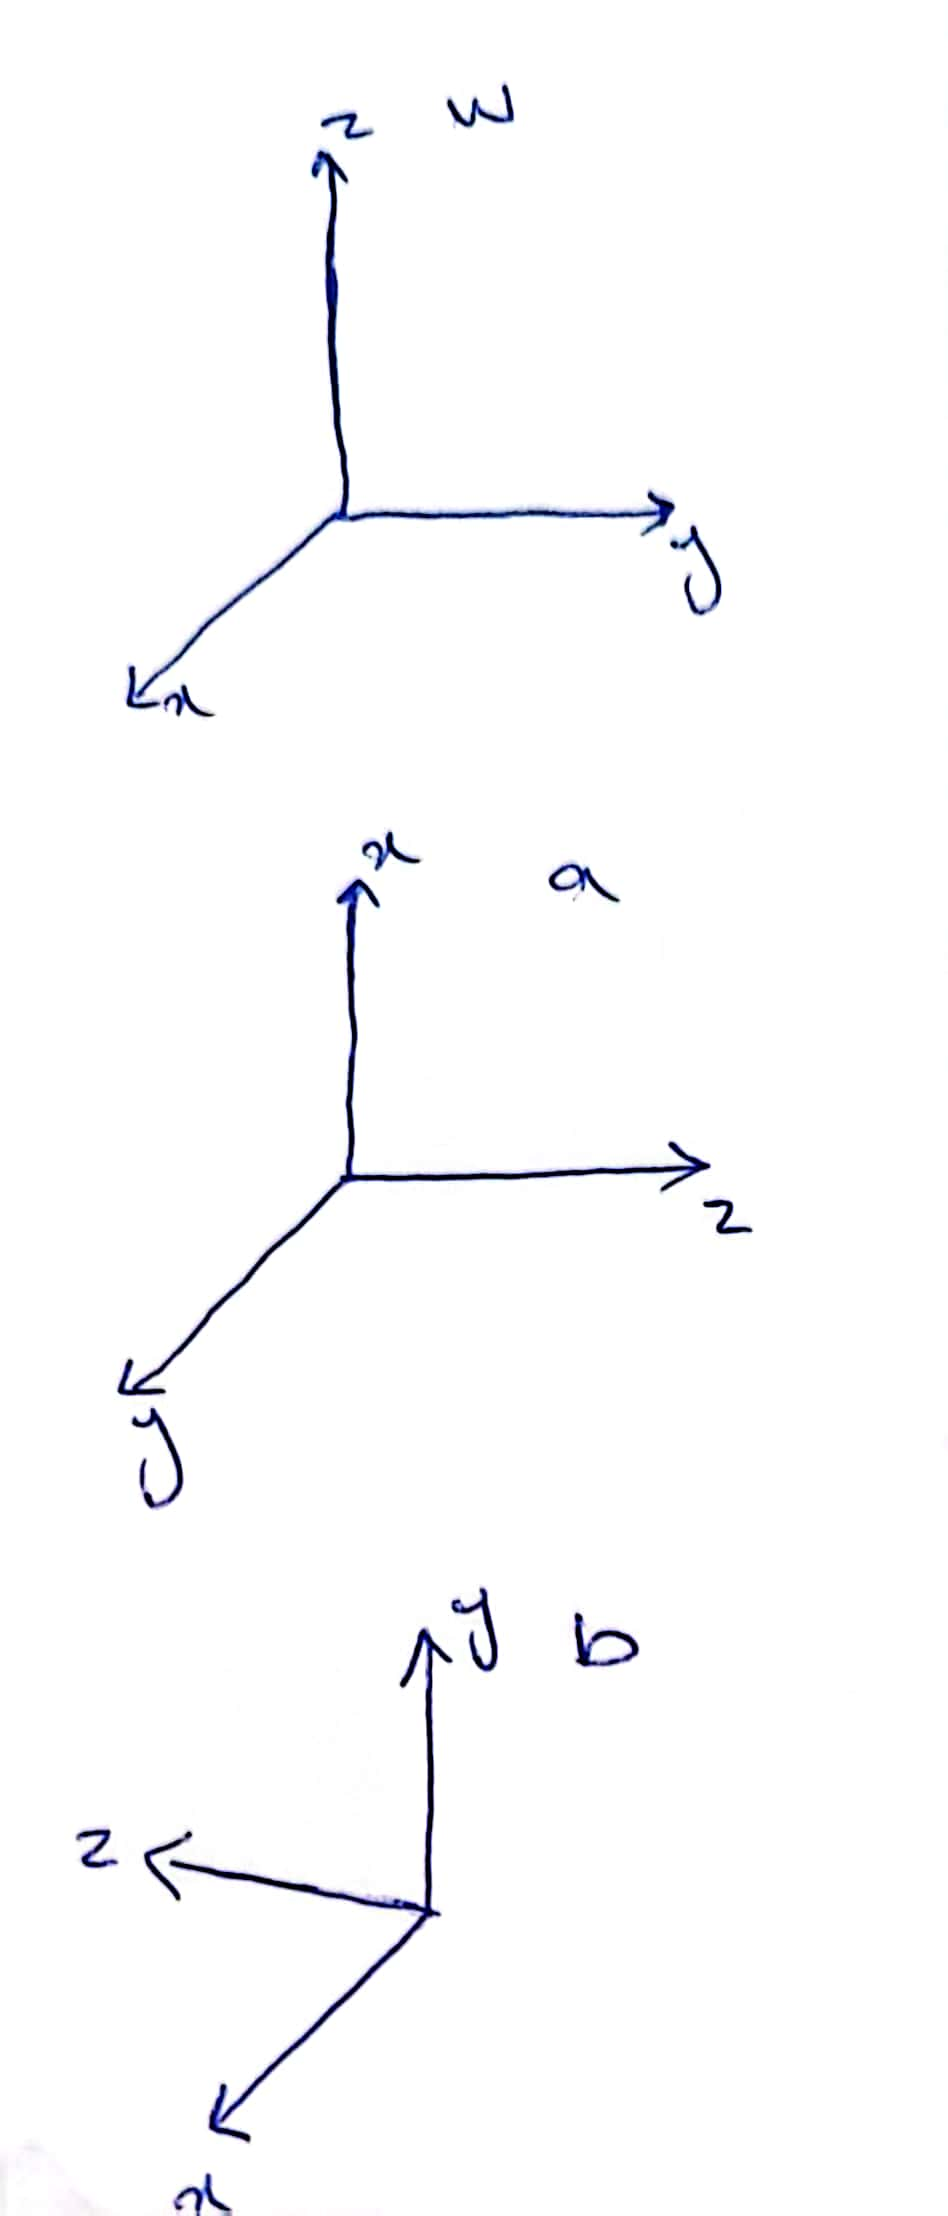
\includegraphics[width=0.3\textwidth]{images/1a.jpg}
        \end{solution}
        \part Part b
        \begin{solution}
            For $R^w_a$, we have to rotate the $y_w$ axis along the $z_w$ axis by $-90^{\circ}$ and the $x_w$ axis along the $y_w$ axis by $-90^{\circ}$.

            \begin{equation*}
                R^w_a = R^w_y(-90^{\circ})R^w_x(-90^{\circ})
            \end{equation*}

            \begin{equation*}
                R^w_a = \begin{bmatrix}
                    cos(-90^{\circ}) & -sin(-90^{\circ}) & 0 \\
                    sin(-90^{\circ}) & cos(-90^{\circ})  & 0 \\
                    0                & 0                 & 1
                \end{bmatrix}
                \begin{bmatrix}
                    cos(-90^{\circ})  & 0 & sin(-90^{\circ}) \\
                    0                 & 1 & 0                \\
                    -sin(-90^{\circ}) & 0 & cos(-90^{\circ})
                \end{bmatrix}
            \end{equation*}

            \begin{equation*}
                R^w_a = \begin{bmatrix}
                    0  & 1 & 0 \\
                    -1 & 0 & 0 \\
                    0  & 0 & 1
                \end{bmatrix}
                \begin{bmatrix}
                    0 & 0 & -1 \\
                    0 & 1 & 0  \\
                    1 & 0 & 0
                \end{bmatrix}
            \end{equation*}

            \begin{equation*}
                R^w_a = \begin{bmatrix}
                    0 & 1 & 0 \\
                    0 & 0 & 1 \\
                    1 & 0 & 0
                \end{bmatrix}
            \end{equation*}

            For $R^w_b$, we have to rotate the world frame along the $x_w$ axis by
            $90^{\circ}$.

            \begin{equation*}
                R^w_b = R^w_x(90^{\circ})
            \end{equation*}

            \begin{equation*}
                R^w_b = \begin{bmatrix}
                    1 & 0               & 0                \\
                    0 & cos(90^{\circ}) & -sin(90^{\circ}) \\
                    0 & sin(90^{\circ}) & cos(90^{\circ})
                \end{bmatrix}
            \end{equation*}

            \begin{equation*}
                R^w_b = \begin{bmatrix}
                    1 & 0 & 0  \\
                    0 & 0 & -1 \\
                    0 & 1 & 0
                \end{bmatrix}
            \end{equation*}
        \end{solution}
        \part Part c
        \begin{solution}
            We can leverage the fact that the rotation matrix is orthogonal and
            that the inverse of an orthogonal matrix is its transpose.

            \begin{equation*}
                (R^w_b)^{-1} = (R^w_b)^T
            \end{equation*}
            \begin{equation*}
                (R^w_b)^{-1} = \begin{bmatrix}
                    1 & 0  & 0 \\
                    0 & 0  & 1 \\
                    0 & -1 & 0
                \end{bmatrix}
            \end{equation*}

            In order to verify that $(R^w_b)^{-1} = (R^w_b)^T$, we can use the inverse to
            transform from the $b$ frame to the $w$ frame.

            $x$-axis in $b$ frame is $[1, 0, 0]^T$.
            \begin{equation*}
                (R^w_b)^{-1} [1, 0, 0]^T = \begin{bmatrix}
                    1 & 0  & 0 \\
                    0 & 0  & 1 \\
                    0 & -1 & 0
                \end{bmatrix}
                \begin{bmatrix}
                    1 \\
                    0 \\
                    0
                \end{bmatrix}
                = \begin{bmatrix}
                    1 \\
                    0 \\
                    0
                \end{bmatrix}
            \end{equation*}

            $y$-axis in $b$ frame is $[0, 0, 1]^T$.
            \begin{equation*}
                (R^w_b)^{-1} [0, 0, 1]^T = \begin{bmatrix}
                    1 & 0  & 0 \\
                    0 & 0  & 1 \\
                    0 & -1 & 0
                \end{bmatrix}
                \begin{bmatrix}
                    0 \\
                    0 \\
                    1
                \end{bmatrix}
                = \begin{bmatrix}
                    0 \\
                    1 \\
                    0
                \end{bmatrix}
            \end{equation*}

            $z$-axis in $b$ frame is $[0, -1, 0]^T$.
            \begin{equation*}
                (R^w_b)^{-1} [0, -1, 0]^T = \begin{bmatrix}
                    1 & 0  & 0 \\
                    0 & 0  & 1 \\
                    0 & -1 & 0
                \end{bmatrix}
                \begin{bmatrix}
                    0  \\
                    -1 \\
                    0
                \end{bmatrix}
                = \begin{bmatrix}
                    0 \\
                    0 \\
                    1
                \end{bmatrix}
            \end{equation*}
            After multiplying the rotation matrix to the frame $b$, we have obtained the
            frame $w$.

        \end{solution}

        \part Part d
        \begin{solution}
            To calculate the rotation matrix $R^a_b$, we can use the following formula:
            \begin{equation*}
                R^a_b = R^a_w R^w_b
            \end{equation*}
            We already have $R^w_b$ and we can get $R^a_w$ by taking the inverse of $R^w_a$.
            \begin{equation*}
                R^a_w = (R^w_a)^{-1} = (R^w_a)^T = \begin{bmatrix}
                    0 & 0 & 1 \\
                    1 & 0 & 0 \\
                    0 & 1 & 0
                \end{bmatrix}
            \end{equation*}
            \begin{equation*}
                R^a_b = \begin{bmatrix}
                    0 & 0 & 1 \\
                    1 & 0 & 0 \\
                    0 & 1 & 0
                \end{bmatrix}
                \begin{bmatrix}
                    1 & 0 & 0  \\
                    0 & 0 & -1 \\
                    0 & 1 & 0
                \end{bmatrix}
                = \begin{bmatrix}
                    0 & 1 & 0  \\
                    1 & 0 & 0  \\
                    0 & 0 & -1
                \end{bmatrix}
            \end{equation*}
            Ans.
        \end{solution}
        \part Part e
        \begin{solution}
            To change the representation of the point ${^b}p = (1, 2, 3)$ to the $w$ frame, we can use the $R^w_b$ rotation matrix.
            \begin{equation*}
                {^w}p = R^w_b {^b}p
            \end{equation*}
            \begin{equation*}
                {^w}p = \begin{bmatrix}
                    1 & 0 & 0  \\
                    0 & 0 & -1 \\
                    0 & 1 & 0
                \end{bmatrix}
                \begin{bmatrix}
                    1 \\
                    2 \\
                    3
                \end{bmatrix}
                = \begin{bmatrix}
                    1  \\
                    -3 \\
                    2
                \end{bmatrix}
            \end{equation*}
        \end{solution}
        \part Part f
        \begin{solution}
            Multiplying the rotation matrix $R^w_b$ with a point in the $b$ frame will change its representation to the $w$ frame.
            Since the point ${^w}p$ is already in the $w$ frame, multiplying it with $R^w_b$ will change its position in the $w$ frame without changing its representation.
            \begin{equation*}
                p = R^w_b {^w}p = \begin{bmatrix}
                    1 & 0 & 0  \\
                    0 & 0 & -1 \\
                    0 & 1 & 0
                \end{bmatrix}
                \begin{bmatrix}
                    1 \\
                    2 \\
                    3
                \end{bmatrix}
            \end{equation*}
            \begin{equation*}
                p = \begin{bmatrix}
                    1  \\
                    -3 \\
                    2
                \end{bmatrix}
            \end{equation*}
            Here $p$ is still in the $w$ frame but its position has changed.

            We can use the rotation matrix $R^b_w$ to change the representation of the
            point ${^w}p$ to the $b$ frame without changing its location.
            \begin{equation*}
                p'' = R^b_w {^w}p = \begin{bmatrix}
                    1 & 0  & 0 \\
                    0 & 0  & 1 \\
                    0 & -1 & 0
                \end{bmatrix}
                \begin{bmatrix}
                    1 \\
                    2 \\
                    3
                \end{bmatrix}
            \end{equation*}
            \begin{equation*}
                p'' = \begin{bmatrix}
                    1 \\
                    3 \\
                    -2
                \end{bmatrix}
            \end{equation*}
            Here $p''$ is in the $b$ frame, so the location is still the same but the representation has changed
            from the $w$ frame to the $b$ frame.
        \end{solution}
        \part Part g
        \begin{solution}
            To change the representation of an angular velocity from frame $w$ to frame $a$, we can use the rotation
            matrix $R^a_w$.
            \begin{equation*}
                {^a}\omega = R^a_w {^w}\omega
                = \begin{bmatrix}
                    0 & 0 & 1 \\
                    1 & 0 & 0 \\
                    0 & 1 & 0
                \end{bmatrix}
                \begin{bmatrix}
                    3 \\
                    2 \\
                    1
                \end{bmatrix}
            \end{equation*}
            \begin{equation*}
                {^a}\omega = \begin{bmatrix}
                    1 \\
                    3 \\
                    2
                \end{bmatrix}
            \end{equation*}
        \end{solution}
    \end{parts}
    \question Problem 2
    \begin{solution}
        We have,
        \begin{equation*}
            r^i_s = r^i_t + r^t_v + r^v_s
        \end{equation*}
        We can differentiate both sides with respect to time with reference to the $i$ frame to get the velocity,
        \begin{equation*}
            v^i_s  =  \dfrac{d}{dt}\Big|_i r^i_t + \frac{d}{dt}\Big|_i r^t_v +\frac{d}{dt}\Big|_i r^v_s
        \end{equation*}
        Using the Coriolis Equation: $\frac{du}{dt}\big|_f  = \frac{du}{dt}\big|_m  + \omega \times u$, we get,
        \begin{equation*}
            v^i_s  = v^i_t +v^t_v + \omega^i_t \times r^t_v + v^v_s + \omega^i_v \times r^v_s
        \end{equation*}
        To get the acceleration, we can differentiate both sides with respect to time with reference to the $i$ frame,
        \begin{equation*}
            a^i_s  =  \dfrac{d}{dt}\Big|_i v^i_t + \frac{d}{dt}\Big|_i v^t_v +\frac{d}{dt}\Big|_i \omega^i_t \times r^t_v +\frac{d}{dt}\Big|_i v^v_s + \frac{d}{dt}\Big|_i \omega^i_v \times r^v_s
        \end{equation*}
        Using the Coriolis Equation again, we get,
        \begin{equation*}
            a^i_s  =  a^i_t + a^t_v + \omega^i_t \times v^t_v + \frac{d}{dt}\Big|_i \omega^i_t \times r^t_v + \frac{d}{dt}\Big|_i r^t_v \times \omega^i_t + a^v_s + \omega^i_v \times v^v_s + \frac{d}{dt}\Big|_i \omega^i_v \times r^v_s + \frac{d}{dt}\Big|_i r^v_s \times \omega^i_v
        \end{equation*}
        Using the fact that the Earth moves with a constant velocity, its acceleration is 0. Therefore, $a^i_t = \frac{d}{dt}\Big|_i \omega^i_t = 0$.

        Similarly, the sensor is fixed to the robot, so its velocity and acceleration
        wrt the robot is 0. Therefore, $v^v_s = a^v_s = 0$.

        Substituting these values in the equation for $a^i_s$, we get,
        \begin{equation*}
            a^i_s  =  a^t_v + \omega^i_t \times v^t_v + (v^t_v + \omega^i_t \times r^t_v) \times \omega^i_t + \frac{d}{dt}\Big|_i \omega^i_v \times r^v_s + (\omega^i_v \times r^v_s) \times \omega^i_v
        \end{equation*}
        Where $\frac{d}{dt}\Big|_i \omega^i_v$ is the angular acceleration of the robot wrt to the center of the Earth. We can write this as $\alpha^i_v$.
    \end{solution}

    \question Problem 3
    \begin{solution}

        The general equation of a steerable wheel is as followed:

        \begin{align*}
            v^w_c = v^w_v + ({\omega}^v_s \times r^s_c) + ({\omega}^w_v \times r^v_c)
        \end{align*}

        Since there is no wheel offset $r^s_c$ will be 0. The equation will be
        simplified as followed:

        \begin{align*}
            v^w_c = v^w_v + ({\omega}^w_v \times r^v_c)
        \end{align*}

        The distance from the wheel to the center of the robot will be considered as l.
        $V_z$ will always be 0 because the robot is constrained to move in x-y plane
        due to the robot always being on the plane.

        \textbf{For wheel 1 where $\alpha_1 = 0^\circ$}

        \begin{equation*}
            \begin{bmatrix}
                V_{1x} \\
                V_{1y} \\
                V_{1z}
            \end{bmatrix}
            = \begin{bmatrix}
                V_x \\
                V_y \\
                0
            \end{bmatrix}
            + \left(\begin{bmatrix}
                0 \\
                0 \\
                \omega
            \end{bmatrix} \times \begin{bmatrix}
                \cos(0) \cdot l \\
                \sin(0) \cdot l \\
                0
            \end{bmatrix}\right)
        \end{equation*}

        \begin{equation*}
            \begin{bmatrix}
                V_{1x} \\
                V_{1y} \\
                V_{1z}
            \end{bmatrix}
            = \begin{bmatrix}
                V_x \\
                V_y \\
                0
            \end{bmatrix}
            + \begin{bmatrix}
                0              \\
                l \cdot \omega \\
                0
            \end{bmatrix}
        \end{equation*}

        \begin{equation} \label{eq:1}
            \begin{bmatrix}
                V_{1x} \\
                V_{1y} \\
                V_{1z}
            \end{bmatrix}
            = \begin{bmatrix}
                V_x                  \\
                V_y + l \cdot \omega \\
                0
            \end{bmatrix}
        \end{equation}

        \textbf{For wheel 2 where $\alpha_1 = 120^\circ$}

        \begin{equation*}
            \begin{bmatrix}
                V_{2x} \\
                V_{2y} \\
                V_{2z}
            \end{bmatrix}
            = \begin{bmatrix}
                V_x \\
                V_y \\
                0
            \end{bmatrix}
            + \left(\begin{bmatrix}
                0 \\
                0 \\
                \omega
            \end{bmatrix} \times \begin{bmatrix}
                \cos(120) \cdot l \\
                \sin(120) \cdot l \\
                0
            \end{bmatrix}\right)
        \end{equation*}

        \begin{equation*}
            \begin{bmatrix}
                V_{2x} \\
                V_{2y} \\
                V_{2z}
            \end{bmatrix}
            = \begin{bmatrix}
                V_x \\
                V_y \\
                0
            \end{bmatrix}
            + \begin{bmatrix}
                - \frac{\sqrt[2]{3}}{2} \cdot l \cdot \omega \\
                - \frac{1}{2} \cdot l \cdot \omega           \\
                0
            \end{bmatrix}
        \end{equation*}

        \begin{equation} \label{eq:2}
            \begin{bmatrix}
                V_{2x} \\
                V_{2y} \\
                V_{2z}
            \end{bmatrix}
            = \begin{bmatrix}
                V_x - \frac{\sqrt[2]{3}}{2} \cdot l \cdot \omega \\
                V_y - \frac{1}{2} \cdot l \cdot \omega           \\
                0
            \end{bmatrix}
        \end{equation}

        \textbf{For wheel 3 where $\alpha_1 = - 120^\circ$}

        \begin{equation*}
            \begin{bmatrix}
                V_{3x} \\
                V_{3y} \\
                V_{3z}
            \end{bmatrix}
            = \begin{bmatrix}
                V_x \\
                V_y \\
                0
            \end{bmatrix}
            + \left(\begin{bmatrix}
                0 \\
                0 \\
                \omega
            \end{bmatrix} \times \begin{bmatrix}
                \cos(- 120) \cdot l \\
                \sin(- 120) \cdot l \\
                0
            \end{bmatrix}\right)
        \end{equation*}

        \begin{equation*}
            \begin{bmatrix}
                V_{3x} \\
                V_{3y} \\
                V_{3z}
            \end{bmatrix}
            = \begin{bmatrix}
                V_x \\
                V_y \\
                0
            \end{bmatrix}
            + \begin{bmatrix}
                \frac{\sqrt[2]{3}}{2} \cdot l \cdot \omega \\
                - \frac{1}{2} \cdot l \cdot \omega         \\
                0
            \end{bmatrix}
        \end{equation*}

        \begin{equation} \label{eq:3}
            \begin{bmatrix}
                V_{3x} \\
                V_{3y} \\
                V_{3z}
            \end{bmatrix}
            = \begin{bmatrix}
                V_x + \frac{\sqrt[2]{3}}{2} \cdot l \cdot \omega \\
                V_y - \frac{1}{2} \cdot l \cdot \omega           \\
                0
            \end{bmatrix}
        \end{equation}

        Equations $\eqref{eq:1}$, $\eqref{eq:2}$, and $\eqref{eq:3}$ represent the
        velocity of contact point of the three wheels in the world frame.

        The steering angles $\beta_i$, where i = 1, 2, 3 are determined by the
        following equations:

        For $\beta_1$:

        $\tan(\beta_1) = \dfrac{V_{1x}}{V_{1y}}$

        $\beta_1 = \tan^{-1}(\dfrac{V_{1x}}{V_{1y}})$

        substituting the subsequent values of $V_{1x}$ and $V_{1y}$ in the above
        equation:

        $\beta_1 = \tan^{-1}(\dfrac{V_x}{V_y + l \cdot \omega})$

        For $\beta_2$:

        $\tan(\beta_2 + 30^\circ) = \dfrac{V_{2y}}{V_{2x}}$

        $\beta_2 = \tan^{-1}(\dfrac{V_{2y}}{V_{2x}}) - 30^\circ$

        substituting the subsequent values of $V_{2x}$ and $V_{2y}$ in the above
        equation:

        $\beta_2 = \tan^{-1}(\dfrac{V_y - \frac{1}{2} \cdot l \cdot \omega}{V_x - \frac{\sqrt[2]{3}}{2} \cdot l \cdot \omega}) - 30^\circ$

        For $\beta_3$:

        $\tan(\beta_3 - 30^\circ) = \dfrac{V_{3y}}{V_{3x}}$

        $\beta_3 = \tan^{-1}(\dfrac{V_{3y}}{V_{3x}}) + 30^\circ$

        substituting the subsequent values of $V_{3x}$ and $V_{3y}$ in the above
        equation:

        $\beta_3 = \tan^{-1}(\dfrac{V_y - \frac{1}{2} \cdot l \cdot \omega}{V_x + \frac{\sqrt[2]{3}}{2} \cdot l \cdot \omega}) + 30^\circ$

    \end{solution}

    \question Problem 4
    \begin{parts}
        \part Part a
        \begin{solution}
            To determine the command that will make the robot move in a clockwise direction in a circle with a radius of 1 unit and return to its starting position, we first need to establish the robot's pose:

            \begin{align*}
                \text{Pose} & = \begin{bmatrix}
                                    1        \\
                                    1        \\
                                    90^\circ \\
                                \end{bmatrix}
            \end{align*}

            The robot's initial position is at coordinates (1, 1) in the world frame, with
            a heading or orientation \(\phi = 90^\circ\). The distance between the robot's
            wheels is 1 unit.

            We can calculate the right and left wheel velocities using the following
            equations:

            \[\text{Right Wheel Velocity:} \quad V_r = (R - \frac{L}{2}) \cdot \omega\]
            \[\text{Left Wheel Velocity:} \quad V_l = (R + \frac{L}{2}) \cdot \omega\]

            Where:
            \begin{itemize}
                \item \(L\) is the distance between the centers of the two wheels.
                \item \(R\) is the signed distance from the Instantaneous Center of Curvature (ICC) to the midpoint between the wheels.
                \item \(\omega\) is the rate of rotation.
            \end{itemize}

            Given that the radius of the circle, \(R\), is 1 unit, we can calculate the
            wheel velocities as follows:

            \begin{align*}
                V_r & = (1 - \frac{1}{2}) \cdot \omega = 0.5 \cdot \omega \\
                V_l & = (1 + \frac{1}{2}) \cdot \omega = 1.5 \cdot \omega
            \end{align*}

            Therefore, the command to make the robot move in this circular path can be
            represented as:

            \[(V_l, V_r, t) = (1.5\cdot\omega, 0.5\cdot\omega, t)\]

            Now, assuming that we want the robot to complete exactly one full clockwise
            rotation before returning to its starting position, we can calculate the time
            duration (\(t\)) required. To do this, we need to determine the distance the
            robot needs to travel, which is equal to the circumference of the circle with a
            radius of 1 unit, \(2\pi\) units.

            Next, we calculate the velocity (\(V\)) of the robot as the average of
            the left and right wheel velocities:

            \[V = \frac{V_l + V_r}{2} = \frac{0.5\omega + 1.5\omega}{2} = \frac{2\omega}{2} = \omega\]

            So, for the given scenario where the robot needs to make one full circle with a
            radius of 1 unit and return to its starting position, you can set the distance to
            \(2\pi\).

            Now, we can calculate the time duration (t) using the formula:

            \[t = \frac{\text{Distance}}{V} = \frac{2\pi}{\omega}\]

            So, to make one full circle and return to the starting position, you can send
            the following command to the robot:

            \[(V_l, V_r, t) = (1.5\cdot\omega, 0.5\cdot\omega, \frac{2\pi}{\omega})\]

            Assuming \(\omega\) to be 1 radian, we can calculate the values of \((V_l, V_r,
            t)\) as follows:

            \begin{align*}
                V_l & = 1.5 \cdot \omega = 1.5 \cdot 1  = 1.5                    \\
                V_r & = 0.5 \cdot \omega = 0.5 \cdot 1  = 0.5                    \\
                t   & = \frac{2\pi}{\omega} = \frac{2\pi}{1 } = 2\pi \, \text{s}
            \end{align*}

            So, assuming \(\omega\) to be 1 radian, we have:

            \[
                (V_l, V_r, t) = (1.5 , 0.5 , 2\pi \, \text{s})
            \]
        \end{solution}
        \part Part b
        \begin{solution}
            Current pose of the robot is given by:
            \begin{align*}
                \text{Pose} & = \begin{bmatrix}
                                    1        \\
                                    1        \\
                                    90^\circ \\
                                \end{bmatrix}
            \end{align*}
            The desired pose of the robot is given by:
            \begin{align*}
                \text{Pose} & = \begin{bmatrix}
                                    3        \\
                                    1        \\
                                    90^\circ \\
                                \end{bmatrix}
            \end{align*}
            We can break our path into two commands, one semi circle and one 180 degree rotation about its center.
            Firstly, we will move our robot along the same path as in part a, but this time we will stop when the robot reaches the point (3, 1) in the world frame. The command for this path is given by:
            \begin{align*}
                (V_l, V_r, t) & = (1.5\cdot\omega, 0.5\cdot\omega, t)
            \end{align*}
            Since we only need to cover half the circle, the distance is $\pi$ instead of $2\pi$ and assuming \(\omega\) to be 1 radian, we can calculate the time duration (t) as follows:
            \begin{align*}
                t & = \frac{\text{Distance}}{V} = \pi
            \end{align*}
            So, to make one semi circle and reach the point (3, 1), you can send the following command to the robot:
            \begin{align*}
                (V_l, V_r, t) & = (1.5, 0.5, \pi)
            \end{align*}
            Now, we need to rotate the robot about its center by 180 degrees. We can calculate the wheel velocities as follows:
            The ICC is the midpoint between the wheels, so $R = 0$.
            \begin{align*}
                V_r & = (0 - \frac{1}{2}) \cdot \omega = - 0.5 \cdot \omega \\
                V_l & = (0 + \frac{1}{2}) \cdot \omega = 0.5 \cdot \omega
            \end{align*}
            The distance to cover is $2\pi r$, $r = L/2 = 0.5$ and since we are rotating by 180 degrees, the distance is $\frac{1}{4} \pi$.
            \begin{align*}
                t & = \frac{\text{Distance}}{V} = \frac{\frac{1}{4} \pi}{\omega}
            \end{align*}
            Assuming \(\omega\) to be 1 radian, we can calculate the values of \((V_l, V_r, t)\) as follows:
            \begin{align*}
                V_l & = 0.5 \cdot \omega = 0.5 \cdot 1  = 0.5                                                     \\
                V_r & = - 0.5 \cdot \omega = - 0.5 \cdot 1  = - 0.5                                               \\
                t   & = \frac{\frac{1}{4} \pi}{\omega} = \frac{\frac{1}{4} \pi}{1 } = \frac{1}{4} \pi \, \text{s}
            \end{align*}
            We can send the following command to the robot:
            \begin{align*}
                (V_l, V_r, t) & = (0.5, - 0.5, \frac{1}{4} \pi)
            \end{align*}
        \end{solution}
        \part Part c
        \begin{solution}
            
        \end{solution}
    \end{parts}
    \question Problem 5
    \begin{parts}
        \part Part a
        \begin{solution}
            abc
        \end{solution}
    \end{parts}

\end{questions}
\end{document}